\documentclass[UTF8]{ctexrep}

\usepackage{fancyhdr}
\usepackage[letterpaper, left=1in, right=1in, top=1in, bottom=1in]{geometry}
\usepackage{sectsty}
\usepackage{graphicx}
\usepackage{subfig}
\usepackage[section]{placeins}
\usepackage{hyperref}
\usepackage{amsmath}
\usepackage{listings}
\usepackage{color}

\definecolor{dkgreen}{rgb}{0,0.6,0}
\definecolor{gray}{rgb}{0.5,0.5,0.5}
\definecolor{mauve}{rgb}{0.58,0,0.82}

\lstset{frame=tb,
    language            = C,
    aboveskip           = 3mm,
    belowskip           = 5mm,
    showstringspaces    = false,
    columns             = flexible,
    basicstyle          = {\small\ttfamily},
    numbers             = none,
    numberstyle         = \tiny\color{gray},
    keywordstyle        = \color{blue},
    commentstyle        = \color{dkgreen},
    stringstyle         = \color{mauve},
    breaklines          = true,
    breakatwhitespace   = true,
    tabsize             = 3,
    numbers             = left,
    numberblanklines    = true,
    firstnumber         = 1,
    numberstyle         = \scriptsize\color{black},
    numbersep           = 12pt,
    escapeinside        = ||,
    mathescape          = true
}
\let\origthelstnumber\thelstnumber
\makeatletter
\newcommand*\Suppressnumber{%
  \lst@AddToHook{OnNewLine}{%
    \let\thelstnumber\relax%
     \advance\c@lstnumber-\@ne\relax%
    }%
}

\newcommand*\Reactivatenumber[1]{%
  \setcounter{lstnumber}{\numexpr#1-1\relax}
  \lst@AddToHook{OnNewLine}{%
   \let\thelstnumber\origthelstnumber%
   \refstepcounter{lstnumber}
  }%
}


\makeatother
\hypersetup{
    colorlinks=true,
    linkcolor=blue,
    filecolor=magenta,
    urlcolor=cyan,
}
\allsectionsfont{\mdseries\scshape}

\renewcommand{\thesection}{\arabic{section}}

\newcommand{\horrule}[1]{\rule{\linewidth}{#1}}
\title{
    \horrule{0.5pt} \\[0.4cm]
    \huge Project 2 \\
    \horrule{2pt}
}
\author{
    陈思贝 (718030290013)
}
\date{
    % TODO: Date
}
\setcounter{section}{-1}

\begin{document}
    \maketitle

    \section{实验配置}

    \begin{itemize}
        \item Linux Kernel: 5.11.16
        \item OS: Ubuntu 18.04.5 LTS
    \end{itemize}
    \vspace{.3cm}

    \section{实验过程}

    \begin{enumerate}
        \item 在\texttt{<include/linux/sched.h>}中合适的位置声明\texttt{ctx}。

        \texttt{task\_struct}前部变量顺序不能随意更改,因此选择在\texttt{randomized\_struct\_fields\_start}后声明\texttt{ctx}。注意不要写在\texttt{\#ifdef}和\texttt{\#endif}之间。
\begin{lstlisting}[firstnumber=649]
    struct task_struct {|\Suppressnumber|
        $\dots$|\Reactivatenumber{664}|
        randomized_struct_fields_start
        int						ctx;        // Declare ctx here |\Suppressnumber|
        $\dots$|\Reactivatenumber{1387}|
    };
\end{lstlisting}

        \item 在\texttt{<kernel/fork.c>}中创建进程时初始化\texttt{ctx=0}。
        
        参考第2526至2550行代码,当\texttt{syscall fork}的时候,调用了\texttt{kernel\_clone(\&args)}。因此定位至第2429行的\texttt{kernel\_clone()},进一步调用了第1852行的\texttt{copy\_process()}。分析代码可得知在第2326行会返回创建成功的子进程,因此只需在此行之前初始化\texttt{ctx}即可。

\begin{lstlisting}[firstnumber=1852]
    static __latent_entropy struct task_struct *copy_process(
            struct pid *pid,
            int trace,
            int node,
            struct kernel_clone_args *args)
    {|\Suppressnumber|
        $\dots$|\Reactivatenumber{2324}|
        copy_oom_score_adj(clone_flags, p);

        p->ctx = 0;     // Initializes ctx to 0
        return p;|\Suppressnumber|
        $\dots$|\Reactivatenumber{2389}|
    }
\end{lstlisting}
        
        \item 在\texttt{<kernel/sched/core.c>}中调度时\texttt{ctx++}。
        
        该文件中\texttt{schedule()}函数负责进程的调度。其中\texttt{tsk}指向当前进程,因此直接在该函数中添加\texttt{ctx++}即可。

\begin{lstlisting}[firstnumber=5145]
asmlinkage __visible void __sched schedule(void)
{
    struct task_struct *tsk = current;

    tsk->ctx++;        // Increments ctx
    sched_submit_work(tsk);|\Suppressnumber|
    $\dots$|\Reactivatenumber{5157}|    
}
\end{lstlisting}

        \item 在\texttt{<fs/proc/base.c>}中创建\texttt{proc entry}。
        
        将\texttt{ctx}的值输出至\texttt{/proc/<pid>/ctx}。\texttt{base.c}文件中的\texttt{tgid\_base\_stuff}记录了目录下创建文件的属性。只需在该数组中添加一条记录即可。因为只需要只读权限,所以\texttt{ONE}宏就满足需求了。同时还需添加一条函数,用于定义读取\texttt{ctx}值的操作。

\begin{lstlisting}[firstnumber=3159]
static int proc_pid_ctx(struct seq_file *m, struct pid_namespace *ns,
			  struct pid *pid, struct task_struct *task)        // Prints ctx value
{
	int err = lock_trace(task);
	if (!err) {
		seq_printf(m, "%d\n", task->ctx);
		unlock_trace(task);
	}
	return err;
}

static const struct pid_entry tgid_base_stuff[] = {|\Suppressnumber|
    $\dots$|\Reactivatenumber{3280}| 
    ONE("ctx", S_IRUSR, proc_pid_ctx),      // Creates ctx file
};
\end{lstlisting}

        \item 编译内核。
        
        参照实验零的步骤,对内核再次进行编译与重新引导,耗时约2小时。使用\texttt{disown -h}指令以防突然断开连接前功尽弃。

        \item 检查实验效果。
        
        编译安装成功后重启设备,并用如下代码生成进程。

\begin{lstlisting}
# include <stdio.h>

int main() {
    while (1) getchar();
    return 0;
}
\end{lstlisting}

        再另开一个终端窗口并用\texttt{cat /proc/<pid>/ctx}查看\texttt{ctx}的值。截图见图\ref{fig:screenshot}。\\
    \end{enumerate}

    \section{实验效果截图}

    \begin{figure}[h!]
        \centering
        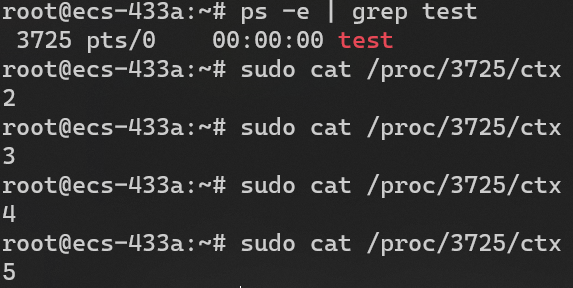
\includegraphics{images/screenshot.png}
        \caption{运行状态截图}
        \label{fig:screenshot}
    \end{figure}

    \section{实验心得}
    这次的代码作业需要对Linux的内核文件程序仔细地研读。对内核程序的流程和其中定义的宏有了更深的理解。与之前的作业不同,内核程序的无法直接修改,更改源文件后,要对内核重新编译,耗时会高达几个小时。所以对于编程准确性要求非常高。同时内核编译中会占用很大的硬盘空间,因此掌握了临时增加磁盘空间的技术。

\end{document}